%% This template can be used to write a paper for
%% Computer Physics Communications using LaTeX.
%% For authors who want to write a computer program description,
%% an example Program Summary is included that only has to be
%% completed and which will give the correct layout in the
%% preprint and the journal.
%% The `elsarticle' style is used and more information on this style
%% can be found at 
%% http://www.elsevier.com/wps/find/authorsview.authors/elsarticle.
%%
%%
\documentclass[preprint,12pt]{elsarticle}

%% Use the option review to obtain double line spacing
%% \documentclass[preprint,review,12pt]{elsarticle}

%% Use the options 1p,twocolumn; 3p; 3p,twocolumn; 5p; or 5p,twocolumn
%% for a journal layout:
% \documentclass[final,1p,times]{elsarticle}
% \documentclass[final,1p,times,twocolumn]{elsarticle}
% \documentclass[final,3p,times]{elsarticle}
% \documentclass[final,3p,times,twocolumn]{elsarticle}
%% \documentclass[final,5p,times]{elsarticle}
% \documentclass[final,5p,times,twocolumn]{elsarticle}

%% if you use PostScript figures in your article
%% use the graphics package for simple commands
%% \usepackage{graphics}
%% or use the graphicx package for more complicated commands
%% \usepackage{graphicx}
%% or use the epsfig package if you prefer to use the old commands
%% \usepackage{epsfig}

%% The amssymb package provides various useful mathematical symbols
\usepackage{amsmath, amssymb, bm}
%% The amsthm package provides extended theorem environments
%% \usepackage{amsthm}

%% The lineno packages adds line numbers. Start line numbering with
%% \begin{linenumbers}, end it with \end{linenumbers}. Or switch it on
%% for the whole article with \linenumbers after \end{frontmatter}.
%% \usepackage{lineno}

%% natbib.sty is loaded by default. However, natbib options can be
%% provided with \biboptions{...} command. Following options are
%% valid:

%%   round  -  round parentheses are used (default)
%%   square -  square brackets are used   [option]
%%   curly  -  curly braces are used      {option}
%%   angle  -  angle brackets are used    <option>
%%   semicolon  -  multiple citations separated by semi-colon
%%   colon  - same as semicolon, an earlier confusion
%%   comma  -  separated by comma
%%   numbers-  selects numerical citations
%%   super  -  numerical citations as superscripts
%%   sort   -  sorts multiple citations according to order in ref. list
%%   sort&compress   -  like sort, but also compresses numerical citations
%%   compress - compresses without sorting
%%
%% \biboptions{comma,round}

% \biboptions{}

%% This list environment is used for the references in the
%% Program Summary
%%
\newcounter{bla}
\newenvironment{refnummer}{%
\list{[\arabic{bla}]}%
{\usecounter{bla}%
 \setlength{\itemindent}{0pt}%
 \setlength{\topsep}{0pt}%
 \setlength{\itemsep}{0pt}%
 \setlength{\labelsep}{2pt}%
 \setlength{\listparindent}{0pt}%
 \settowidth{\labelwidth}{[9]}%
 \setlength{\leftmargin}{\labelwidth}%
 \addtolength{\leftmargin}{\labelsep}%
 \setlength{\rightmargin}{0pt}}}
 {\endlist}
\usepackage{subcaption}
\usepackage[newfloat]{minted}
\usepackage{hyperref}
\usepackage{tcolorbox}
\usepackage{etoolbox}
\BeforeBeginEnvironment{minted}{\begin{tcolorbox}}
\AfterEndEnvironment{minted}{\end{tcolorbox}}
\usepackage{caption}

\newenvironment{code}{\captionsetup{type=listing}}{}
\SetupFloatingEnvironment{listing}{name=Code Block}

\newcommand{\SuperScreen}{\mintinline{python}{SuperScreen}\,}

\journal{Computer Physics Communications}

\begin{document}

\begin{frontmatter}

%% Title, authors and addresses

%% use the tnoteref command within \title for footnotes;
%% use the tnotetext command for the associated footnote;
%% use the fnref command within \author or \address for footnotes;
%% use the fntext command for the associated footnote;
%% use the corref command within \author for corresponding author footnotes;
%% use the cortext command for the associated footnote;
%% use the ead command for the email address,
%% and the form \ead[url] for the home page:
%%
%% \title{Title\tnoteref{label1}}
%% \tnotetext[label1]{}
%% \author{Name\corref{cor1}\fnref{label2}}
%% \ead{email address}
%% \ead[url]{home page}
%% \fntext[label2]{}
%% \cortext[cor1]{}
%% \address{Address\fnref{label3}}
%% \fntext[label3]{}

\title{\texttt{SuperScreen}: An open-source package for simulating the magnetic response of 2D superconductors}

%% use optional labels to link authors explicitly to addresses:
%% \author[label1,label2]{<author name>}
%% \address[label1]{<address>}
%% \address[label2]{<address>}

\author[a]{Logan Bishop-Van Horn}
\author[a,b]{Kam Moler\corref{author}}

\cortext[author]{Corresponding author.\\\textit{E-mail address:} kmoler@stanford.edu}
\address[a]{First Address}
\address[b]{Second Address}

\begin{abstract}
%% Text of abstract
A submitted program is expected to satisfy the following criteria: it must be of benefit to other physicists, or be an exemplar of good programming practice, or illustrate new or novel programming techniques which are of importance to computational physics community; it should be implemented in a language and executable on hardware that is widely available and well documented; it should meet accepted standards for scientific programming; it should be adequately documented and, where appropriate, supplied with a separate User Manual, which together with the manuscript should make clear the structure, functionality, installation, and operation of the program.

Your manuscript and figure sources should be submitted through Editorial Manager (EM) by using the online submission tool at \\
https://www.editorialmanager.com/comphy/.

In addition to the manuscript you must supply: the program source code; a README file giving the names and a brief description of the files/directory structure that make up the package and clear instructions on the installation and execution of the program; sample input and output data for at least one comprehensive test run; and, where appropriate, a user manual.

A compressed archive program file or files, containing these items, should be uploaded at the "Attach Files" stage of the EM submission.

For files larger than 1Gb, if difficulties are encountered during upload the author should contact the Technical Editor at cpc.mendeley@gmail.com.

\end{abstract}

\begin{keyword}
%% keywords here, in the form: keyword \sep keyword
keyword1; keyword2; keyword3; etc.

\end{keyword}

\end{frontmatter}

%%
%% Start line numbering here if you want
%%
% \linenumbers

% All CPiP articles must contain the following
% PROGRAM SUMMARY.
\noindent
{\bf PROGRAM SUMMARY}

\begin{small}
\noindent
{\em SuperScreen:}\\
{\em CPC Library link to program files:} (to be added by Technical Editor) \\
{\em Developer's repository link:} \href{http://www.github.com/loganbvh/superscreen}{www.github.com/loganbvh/superscreen}\\
{\em Code Ocean capsule:} (to be added by Technical Editor)\\
{\em Licensing provisions:} MIT\\
{\em Programming language: Python}\\
{\em Supplementary material:}\\
  % Fill in if necessary, otherwise leave out.
% {\em Journal reference of previous version:}*\\
  %Only required for a New Version summary, otherwise leave out.
% {\em Does the new version supersede the previous version?:}*\\
  %Only required for a New Version summary, otherwise leave out.
% {\em Reasons for the new version:*}\\
  %Only required for a New Version summary, otherwise leave out.
% {\em Summary of revisions:}*\\
  %Only required for a New Version summary, otherwise leave out.
{\em Nature of problem(approx. 50-250 words):}\\
  %Describe the nature of the problem here. \\
{\em Solution method(approx. 50-250 words):}\\
  %Describe the method solution here.
{\em Additional comments including restrictions and unusual features (approx. 50-250 words):}\\
  %Provide any additional comments here.
   \\

% \begin{thebibliography}{0}
% \bibitem{1}Reference 1         % This list should only contain those items referenced in the                 
% \bibitem{2}Reference 2         % Program Summary section.   
% \bibitem{3}Reference 3         % Type references in text as [1], [2], etc.
%                               % This list is different from the bibliography at the end of 
%                               % the Long Write-Up.
% \end{thebibliography}
\end{small}


%% main text
\section{Introduction}
\label{section:introduction}

\SuperScreen is an open-source Python package developed to simulate the magnetic response of structures composed of one or more layers containing superconducting thin films. \SuperScreen solves the coupled Maxwell's and London's equations in and around superconducting films with spatially-varying penetration depth in the presence of applied magnetic fields and trapped flux using a matrix inversion method introduced by Brandt~\cite{brandt_thin_2005} and initially implemented by Kirtley, \emph{et al.}~\cite{kirtley_scanning_2016, kirtley_response_2016} to model the magnetic response of scanning superconducting quantum interference device (SQUID) sensors.

In Section~\ref{section:model} we outline Brandt's model, and in Section~\ref{section:implementation} we describe its numerical implementation. In Section~\ref{section:overview}, we provide an overview of the structure of the \SuperScreen package, highlighting notable functions, classes, and features, and discuss some important development details. In Section~\ref{section:examples}, we demonstrate how to set up and solve several types of models using \SuperScreen. Finally, in Section~\ref{section:conlusion} we discuss potential applications, extensions, and improvements to the package.

\section{The Model}
\label{section:model}

The goal of \SuperScreen is to model the magnetic response of a thin superconducting film, or a structure composed of multiple superconducting films (which may or may not lie in the same plane), to an applied inhomogeneous out-of-plane magnetic field
$H_{z,\,\mathrm{applied}}(x, y, z)$.

Given $H_{z,\,\mathrm{applied}}(x, y, z)$ and information about the geometry and magnetic penetration depth of all films in a superconducting structure, we aim to calculate the thickness-integrated current density (or sheet current) $\vec{J}(x, y)$ at all points inside the films, from which one can calculate the vector magnetic field $\vec{H}(x, y, z)$ at all points both inside and outside the films.

A convenient method for solving this problem was introduced by Brandt in~\cite{brandt_thin_2005}, and subsequently used to model the magnetic response of scanning Superconducting Quantum Interference Device (SQUID) susceptometers~\cite{kirtley_scanning_2016, kirtley_response_2016}.

In the London model of superconductivity, the magnetic field $\vec{H}(\vec{r})$ and 3D current density $\vec{j}(\vec{r})$ in a superconductor with London penetration depth $\lambda(\vec{r})$ obey the second London equation:
$\nabla\times\vec{j}(\vec{r})=-\vec{H}(\vec{r})/\lambda^2(\vec{r})$, where
$\nabla=\left(\frac{\partial}{\partial x}, \frac{\partial}{\partial y}, \frac{\partial}{\partial z}\right)$. Brandt's model assumes that the current density $\vec{j}$ is approximately independent of $z$, such $\vec{j}(\vec{r}) = \vec{j}(x, y, z)\approx\vec{j}_{z_0}(x, y)$ for a film lying parallel to the $x-y$ plane at vertical position $z_0$. Working now with the thickness-integrated current density (sheet current) $\vec{J}(x, y)\approx\vec{j}_{z_0}(x, y)\cdot d$, where $d$
is the thickness of the film, the second London equation reduces to

\begin{equation}
    \label{eq:london}
    \nabla\times\vec{J}(x, y)=-\vec{H}(x, y)/\Lambda(x, y),
\end{equation}
where $\Lambda(x, y)=\lambda^2(x, y)/d$ is the effective penetration depth
of the superconducting film (equal to half the Pearl length~\cite{pearl_current_1964}).

It is important to note that the assumption $\vec{j}(x, y, z)\approx\vec{j}_{z_0}(x, y)$ is valid for only films that are thinner than their London penetration depth ($d<\lambda$, such that $\Lambda=\lambda^2/d>\lambda$). However the model has been applied with some success in structures with $\lambda\lesssim d$~\cite{kirtley_scanning_2016,kirtley_response_2016}. Aside from this limitation, the method described below can in principle to used to model films with any effective penetration depth $0\leq\Lambda<\infty$.

Because the sheet current has zero divergence in the superconducting film ($\nabla\cdot\vec{J}=0$)
except at small contacts where current can be injected, one can express the sheet current in terms
of a scalar potential $g(x, y)$, called the stream function:

\begin{equation}
    \label{eq:stream}
    \vec{J}(x, y) = -\hat{z}\times\nabla g
    = \nabla\times(g\hat{z})
    = \left(\frac{\partial g}{\partial y}, -\frac{\partial g}{\partial x}\right).
\end{equation}

The stream function $g$ can be thought of as the local magnetization of the film, or the area density of magnetic dipole sources (see \cite{brandt_thin_2005} for more interesting properties of the stream function). We can re-write Eq.~\ref{eq:london} for a 2D film in terms of $g$:

\begin{align}
    \label{eq:london_stream}
    \begin{split}
        \vec{H}(x, y) &= -\Lambda\left[\nabla\times\vec{J}(x, y)\right]\\
        &= -\Lambda\left[\nabla\times\left(\nabla\times(g\hat{z})\right)\right]\\
        &= -\Lambda\left[\nabla(\nabla\cdot(g\hat{z}))-\nabla^2(g\hat{z})\right]\\
        &=\Lambda\nabla^2g(x,y)\hat{z}\\
        &=H_z(x, y)\hat{z}
    \end{split}
\end{align}
where $\nabla^2=\nabla\cdot\nabla$ is the Laplace operator. (The fourth line follows from the fact that $\nabla\cdot\left[g(x,y)\hat{z}\right] = 0$). From Ampere's Law, the three components of the magnetic field at position $\vec{r}=(x, y, z)$ due to a sheet of current lying in the $x-y$ plane (at vertical position $z'$) with stream function $g(x', y')$ are given by:

\begin{align}
    \label{eq:field_from_kernel}
    \begin{split}
        H_x(\vec{r}) &= \int_S Q_x(\vec{r},\vec{r}')g(x', y')\,\mathrm{d}^2r'\\
        H_y(\vec{r}) &= \int_S Q_y(\vec{r},\vec{r}')g(x', y')\,\mathrm{d}^2r'\\
        H_z(\vec{r}) &= H_{z,\,\mathrm{applied}}(\vec{r})
        + \int_S Q_z(\vec{r},\vec{r}')g(x', y')\,\mathrm{d}^2r'  
    \end{split}
\end{align}

Here we assume an out-of-plane applied magnetic field $\vec{H}_\mathrm{applied}(\vec{r}')=H_\mathrm{z,\,\mathrm{applied}}(\vec{r}')\hat{z}$. $S$ is the film area (with $g = 0$ outside of the film), and $Q_x(\vec{r},\vec{r}')$, $Q_y(\vec{r},\vec{r}')$, and $Q_z(\vec{r},\vec{r}')$ are dipole kernel functions which give the relevant component of the magnetic field at position $\vec{r}=(x, y, z)$ due to a dipole of unit strength at position $\vec{r}'=(x', y', z')$:

\begin{align}
    \label{eq:kernels}
    \begin{split}
        Q_x(\vec{r}, \vec{r}') &=  3\frac{(x-x')(z-z')}
        {4\pi[(z-z')^2+\rho^2]^{5/2}}\\
        Q_y(\vec{r}, \vec{r}') &=  3\frac{(y-y')(z-z')}
        {4\pi[(z-z')^2+\rho^2]^{5/2}}\\
        Q_z(\vec{r}, \vec{r}') &=  \frac{2(z-z')^2-\rho^2}
        {4\pi[(z-z')^2+\rho^2]^{5/2}},
    \end{split}
\end{align}
where $\rho=\sqrt{(x-x')^2 + (y-y')^2}$.

Comparing Eq.~\ref{eq:london_stream} and Eq.~\ref{eq:field_from_kernel}, we have in the plane of the film:

\begin{align}
    \label{eq:integral_equation}
    \begin{split}
        \underbrace{H_z(\vec{r}) = \vec{H}(\vec{r})\cdot\hat{z}
        = \Lambda\nabla^2g(x, y)}_{z-\text{component of the total field}}
        = \underbrace{H_{z,\,\mathrm{applied}}(\vec{r})}_{\text{applied field}}
        + \underbrace{\int_S Q_z(\vec{r},\vec{r}')g(\vec{r}')\,\mathrm{d}^2r'}_{\text{screening field}},
    \end{split}
\end{align}
(where now $\vec{r}$ and $\vec{r}'$ are 2D vectors, i.e. $\Delta z=0$, since the film is in the same plane as itself). From Eq.~\ref{eq:integral_equation}, we arrive at an integral equation relating the stream function $g$ for points inside the superconductor to the applied field $H_{z,\,\mathrm{applied}}$:

\begin{equation}
    \label{eq:applied_to_stream}
    H_{z,\,\mathrm{applied}}(\vec{r})
    = -\int_S\left[
        Q_z(\vec{r},\vec{r}')-\delta(\vec{r}-\vec{r}')\Lambda(\vec{r}')\nabla^2\right
    ]g(\vec{r}')\,\mathrm{d}^2r'
\end{equation}

The goal, then, is to solve (invert) Eq.~\ref{eq:applied_to_stream} for a given $H_{z,\,\mathrm{applied}}$ and film geometry $S$ to obtain $g$ for all points inside the film (with $g=0$ enforced outside the film). Once $g(\vec{r})$ is known, the full vector magnetic field $\vec{H}(\vec{r})$ can be calculated at any point $\vec{r}$
from Eqs.~\ref{eq:field_from_kernel} and \ref{eq:kernels}.

\subsection{Films with holes}
\label{section:model:holes}

In films that have holes (regions of vacuum completely surrounded by superconductor), each hole $k$ can contain a trapped flux $\Phi_k$, with an associated circulating current $I_{\mathrm{circ},\,k}$. The (hypothetical) applied field that would cause such a circulating current is given by Eq.~\ref{eq:applied_to_stream} if we set $g(\vec{r})=I_{\mathrm{circ},\,k}$ for all points $\vec{r}$ lying inside hole $k$:

\begin{equation}
    \label{eq:Heff}
    H_{z,\,\mathrm{eff},\,k}(\vec{r}) = -\int_{\mathrm{hole}\,k}[
        Q_z(\vec{r},\vec{r}')-\Lambda(\vec{r}')\nabla^2
    ] I_{\mathrm{circ},\,k} \,\mathrm{d}^2r'.   
\end{equation}

In this case, we modify the left-hand side of Eq.~\ref{eq:applied_to_stream} as follows:

\begin{equation}
    \label{eq:Heff_sub}
    H_{z,\,\mathrm{applied}}(\vec{r}) - \sum_{\mathrm{holes}\,k} H_{z,\,\mathrm{eff},\,k}(\vec{r})
    = -\int_S\left[
        Q_z(\vec{r},\vec{r}')-\delta(\vec{r}-\vec{r}')\Lambda(\vec{r}')\nabla^2\right
    ]g(\vec{r}')\,\mathrm{d}^2r'.
\end{equation}

\subsection{Multi-layer structures}
\label{section:model:multilayer}

For structures with multiple films lying in different planes or layers, with layer $\ell$ lying in the plane $z=z_\ell$,
the stream functions and fields for all layers can be computed self-consistently using the following recipe:

\begin{enumerate}
    \item{
        Calculate the stream function $g_\ell(\vec{r})$ for each layer $\ell$ by solving Eq.~\ref{eq:Heff_sub} given an applied field $H_{z,\,\mathrm{applied}}(\vec{r}, z_\ell)$.
    }
    \item{
        For each layer $\ell$, calculate the $z$-component of the field due to the currents in all other layers $m\neq\ell$ (encoded in the stream function $g_m(\vec{r})$)
        using Eq.~\ref{eq:field_from_kernel}.
    }
    \item{
        Re-solve Eq.~\ref{eq:Heff_sub} taking the new applied field at each layer to be the original applied field plus the sum of screening fields from all other layers. This is accomplished via the substitution
        $$
            H_{z,\,\mathrm{applied}}(\vec{r}, z_\ell) \to
            H_{z,\,\mathrm{applied}}(\vec{r}, z_\ell)
            + \sum_{m\neq\ell}
            \int_S Q_z(\vec{r},\vec{r}')g_m(\vec{r}')\,\mathrm{d}^2r.
        $$
    }
    \item{
        Repeat steps 1-3 until the solution converges.
    }
\end{enumerate}

Convergence can be quantified by, for example, calculating the total magnetic flux though all films and holes in the model at the end of each iteration.

\section{Numerical Implementation}
\label{section:implementation}

In order to numerically solve Eq.~\ref{eq:field_from_kernel} and Eq.~\ref{eq:Heff_sub}, we have to discretize the films, holes, and the vacuum regions surrounding them. We use a triangular
(Delaunay) mesh, consisting of $n$ points (or vertices)
which together form $m$ triangles. Below we denote column vectors and matrices using bold font. $\mathbf{A}\mathbf{B}$
denotes matrix multiplication, with $(\mathbf{A}\mathbf{B})_{ij}=\sum_{k=1}^\ell A_{ik}B_{kj}$
($\ell$ being the number of columns in $\mathbf{A}$ and the number of rows in $\mathbf{B}$). Column vectors are treated as matrices with $\ell$ rows and 1 column. On the other hand, we denote element-wise multiplication with a dot: $(\mathbf{A}\cdot\mathbf{B})_{ij}=A_{ij}B_{ij}$ for two matrices
and $(\mathbf{A}\cdot\mathbf{v})_{ij}=(\mathbf{v}\cdot\mathbf{A})_{ij}=A_{ij}v_{i}$ for a matrix $\mathbf{A}$ and a column vector $\mathbf{v}$.

The matrix version of Eq.~\ref{eq:field_from_kernel} is:

\begin{equation}
    \label{eq:field_from_kernel_num}
    \underbrace{\mathbf{h}_z}_\text{total field}
    = \underbrace{\mathbf{h}_{z,\,\mathrm{applied}}}_\text{applied field}
    + \underbrace{(\mathbf{Q}\cdot\mathbf{w})\mathbf{g}}_\text{screening field}.
\end{equation}

The kernel matrix $\mathbf{Q}$ and weight matrix $\mathbf{w}$ together play the role of the
kernel function $Q_z(\vec{r},\vec{r}')$ for all points lying in the plane of the film. They are both $n\times n$ matrices determined solely by the geometry of the mesh.
$\mathbf{h}_z$, $\mathbf{h}_{z,\,\mathrm{applied}}$, and $\mathbf{g}$ are all $n\times 1$ vectors, with each row representing the value of the quantity at the
corresponding vertex in the mesh. There are several different methods for constructing the weight matrix $\mathbf{w}$, which are discussed in Section~\ref{section:implementation:laplace} below. The kernel
matrix $\mathbf{Q}$ is defined in terms of a matrix $\mathbf{q}$ with
$q_{ij} = \left(4\pi|\vec{r}_i-\vec{r}_j|^3\right)^{-1}$
(which is $\lim_{\Delta z\to 0}Q_z(\vec{r},\vec{r}')$ cf. Eq.~\ref{eq:kernels}),
and a vector $\mathbf{C}$:

\begin{equation}
    \label{eq:kernel_matrix}
    Q_{ij} = (\delta_{ij}-1)q_{ij}
    + \delta_{ij}\frac{1}{w_{ij}}\left(C_i + \sum_{l\neq i}q_{il}w_{il}\right),
\end{equation}
where $\delta_{ij}$ is the Kronecker delta function. The diagonal terms involving $\mathbf{C}$ are meant to work around the fact that $q_{ii}$ diverge (see \cite{brandt_thin_2005} for more details), and the vector is defined as

\begin{equation}
    \label{eq:C_vector}
    C_i = \frac{1}{4\pi}\sum_{p,q=\pm1}\sqrt{[\Delta x - p(x_i-\bar{x})]^{-2} + [\Delta y - q(y_i-\bar{y})]^{-2}},
\end{equation}
where $\Delta x=(x_\mathrm{max}-x_\mathrm{min})/2$ and $\Delta y=(y_\mathrm{max}-y_\mathrm{min})/2$ are half the side lengths of a rectangle bounding the modeled film and $(\bar{x}, \bar{y})$ are the coordinates of the center of the rectangle.

The matrix version of Eq.~\ref{eq:Heff_sub} is:

\begin{equation}
    \label{eq:Heff_sub_num}
     \mathbf{h}_{z,\,\mathrm{applied}} - \sum_{\mathrm{holes}\, k}\mathbf{h}_{z,\,\mathrm{eff},\,k} = -(\mathbf{Q}\cdot\mathbf{w}-\mathbf{\Lambda}\cdot\mathbf{\nabla}^2)\mathbf{g},
\end{equation}
where we exclude points in the mesh lying outside of the superconducting film but keep points
inside holes in the film. $\mathbf{\Lambda}$ is either a scalar or a vector defining the effective penetration depth at every included vertex in the mesh, and $\mathbf{\nabla}^2$
is the Laplace operator, an $n\times n$ matrix defined such that $\mathbf{\nabla}^2\mathbf{f}$ computes the Laplacian $\nabla^2f(x,y)$ of a function $f(x,y)$ defined on the mesh  (see Section~\ref{section:implementation:laplace}).

Eq.~\ref{eq:Heff_sub_num} is a matrix equation relating the applied field to the stream function
inside a superconducting film, which can efficiently be solved (e.g. by matrix inversion or LU decomposition) for the unknown vector $\mathbf{g}$, the stream function inside the film. Since the stream function outside the film and inside holes in the film is already known, solving Eq.~\ref{eq:Heff_sub_num} gives us the stream function for the full mesh:

\begin{equation}
    \label{eq:full_stream}
    \mathbf{g} = \begin{cases}
        \left(-[\mathbf{Q}\cdot\mathbf{w}-\mathbf{\Lambda}\cdot\mathbf{\nabla}^2]\right)^{-1}
        \left(\mathbf{h}_{z,\,\mathrm{applied}} - \sum_{\mathrm{holes}\,k}\mathbf{h}_{z,\,\mathrm{eff},\,k}\right)
            & \text{inside the film}\\
        I_{\mathrm{circ},\,k}
            & \text{inside hole }k\\
        0
            & \text{elsewhere}
    \end{cases}
\end{equation}

Once the stream function $\mathbf{g}$ is known for the full mesh,
the sheet current flowing in the film can be computed from Eq.~\ref{eq:stream}, the $z$-component of the total field in the plane of the film can be computed
from Eq.~\ref{eq:field_from_kernel_num}, and the full vector magnetic field $\vec{H}(x, y, z)$
at any point in space can be computed from Eq.~\ref{eq:field_from_kernel}.

\subsection{Laplace operator}
\label{section:implementation:laplace}

The definition of the discrete Laplace operator $\mathbf{\nabla}^2$ (also called the Laplace-Beltrami operator) deserves special attention, as it reduces the problem of solving a partial differential equation $\nabla^2g(x,y)=f(x,y)$ to the problem of solving a matrix equation
$\mathbf{\nabla}^2\mathbf{g}=\mathbf{f}$~\cite{Reuter_Biasotti_Giorgi_Patane_Spagnuolo_2009}. As described in [Vaillant-Laplacian-2013] and [Laplacian-SGP-2014] the Laplace operator $\mathbf{\nabla}^2$ for a mesh is defined in terms of two matrices, the mass matrix $\mathbf{M}$ and the
weak Laplacian matrix $\mathbf{L}$: $\mathbf{\nabla}^2 = \mathbf{M}^{-1}\mathbf{L}$.


In a 2D mesh, the mass matrix $\mathbf{M}$ gives an effective area to each vertex in the mesh. Here we use a ``lumped" mass matrix, which is diagonal with elements $M_{ii} = \frac{1}{3}\sum_{t\in\mathcal{N}(i)}\mathrm{area}(t)$,
where $\mathcal{N}(i)$ is the set of triangles $t$ adjacent to vertex $i$. The weak Laplacian matrix $\mathbf{L}$ is defined in terms of a symmetric weight matrix $\mathbf{W}$, which assigns a weight to every edge in the mesh. $\mathbf{W}$ may be defined in a number of ways:

\begin{enumerate}
    \item{
        Uniform weighting: In this case, $\mathbf{W}$ is simply the adjacency matrix for the mesh vertices:
        $$
            W_{ij} =
            \begin{cases}
                0&\text{if }i=j\\
                1&\text{if }i\text{ is adjacent to }j\\
                0&\text{otherwise}
            \end{cases}
        $$
    }
    \item{
        Inverse-Euclidean weighting: Each edge is weighted by the inverse of its length: $|\vec{r}_i-\vec{r}_j|^{-1}$, where $\vec{r}_i$ is the position of vertex $i$.
        $$
            W_{ij} =
            \begin{cases}
                0&\text{if }i=j\\
                |\vec{r}_i-\vec{r}_j|^{-1}&\text{if }i\text{ is adjacent to }j\\
                0&\text{otherwise}
            \end{cases}
        $$
    }
    \item{
        Half-cotangent weighting: Each edge is weighted by the half the sum of the cotangents of the two angles opposite to it.
        $$
            W_{ij} =
            \begin{cases}
                0&\text{if }i=j\\
                \frac{1}{2}\left(\cot\alpha_{ij}+\cot\beta_{ij}\right)&\text{if }i\text{ is adjacent to }j\\
                0&\text{otherwise}
            \end{cases}
        $$
    }
\end{enumerate}

By default, \SuperScreen uses half-cotangent weighting. The Laplacian matrix $\mathbf{C}$ is defined in terms of the weight matrix $\mathbf{W}$: $L_{ij} = W_{ij} - \delta_{ij}\sum_{\ell}W_{i\ell}$. Finally, the Laplace operator is given by $\mathbf{\nabla}^2 = \mathbf{M}^{-1}\mathbf{L}$.

The matrix $\mathbf{w}$ in Eqs.~\ref{eq:field_from_kernel_num} and \ref{eq:Heff_sub_num} that is used, together with the kernel matrix $\mathbf{Q}$, to approximate the dipole kernel $Q_z(\vec{r},\vec{r}')$ (Eq.~\ref{eq:kernels}) is simply a normalized version of the weight matrix $\mathbf{W}$ used in defining the Laplace operator. The relationship between $\mathbf{w}$ and $\mathbf{W}$ is given by:
$$
    w_{ij} = \begin{cases}
        1&\text{if }i = j\\
        W_{ij} / \sum_{i\neq j} W_{ij}&\text{otherwise}
    \end{cases}
$$

\section{Package Overview}
\label{section:overview}

In this section we give a high-level overview of the \SuperScreen package. More detailed documentation and tutorials can be found at \href{http://www.superscreen.readthedocs.io}{www.superscreen.readthedocs.io}.

\subsection{Parameters}
\label{section:overview:parameter}

A \mintinline{python}{superscreen.Parameter} is a wrapper around a Python function that computes a scalar value as a function of position coordinates ($x$, $y$, and optionally $z$) based on some set of keyword arguments. Addition, subtraction, multiplication, division, and exponentiation between \mintinline{python}{Parameters}, other \mintinline{python}{Parameters}, and Python scalars (\mintinline{python}{int} and \mintinline{python}{float}) are supported. For example, see Code Block~\ref{code:parameters}.

\begin{code}
\begin{minted}[fontsize=\footnotesize]{python}
from superscreen import Parameter

def f(x, y, a=1, b=0):
    return a * x**2 + b * y
    
param = Parameter(f, a=0, b=1)
print(param)
# Parameter<f(a=0, b=1)>

other_param = Parameter(f, a=2, b=3)
print(other_param)
# Parameter<f(a=2, b=3)>

print(param(0, 0) == f(0, 0, a=0, b=1))
# True
print(other_param(1, 2) == f(1, 2, a=2, b=3))
# True

param_squared = param ** 2
print(param_squared)
# CompositeParameter<(f(a=0, b=1) ** 2)>

print(param_squared(3, 4) == f(3, 4, a=0, b=1) ** 2)
# True
print(
    (5 * param_squared / other_param)(5, 6)
    == 5 * f(5, 6, a=0, b=1) ** 2 / f(5, 6, a=2, b=3)
)
# True
\end{minted}
\captionof{listing}{The basic usage of \mintinline{python}{Parameters}. \mintinline{python}{Parameters} can be used to conveniently define applied magnetic fields and penetration depths that depend on position.}
\label{code:parameters}
\end{code}

\subsection{Devices}
\label{section:overview:device}

Information about the geometry and penetration depth of a superconducting structure is described by an instance of the \mintinline{python}{superscreen.Device} class. A \mintinline{python}{Device} is made up of one or more superconducting layers, each an instance of  \mintinline{python}{superscreen.Layer}. Each layer sits in a specified plane parallel to the $x-y$ plane and has its own effective penetration depth $\Lambda$, which can either be a constant or a \mintinline{python}{superscreen.Parameter} that defines $\Lambda(x, y)$, the effective penetration depth as a function of position. The effective penetration depth $\Lambda$ can instead be defined in terms of a layer's London penetration depth $\lambda$ and its thickness $d$: $\Lambda=\lambda^2/d$, in which case the London penetration depth can be either a constant or a \mintinline{python}{superscreen.Parameter}.

Each layer can contain one or more superconducting films which may have one or more holes in them. Films and holes are represented by instances of the \mintinline{python}{superscreen.Polygon} class. A \mintinline{python}{Polygon} contains the name of the layer to which is belongs, an array specifying the coordinates of its vertices, and a method, \mintinline{python}{Polygon.contains_points()}, which determines whether specified coordinates lie within the polygon or not. In addition to superconducting films and holes, one may define ``abstract regions,'' which are polygons that need not correspond to a physical feature in the structure, but will still be meshed. Abstract regions can be used to define a ``bounding box" around a structure. The \mintinline{python}{superscreen.geometry} module provides functions for generating the underlying polygon vertices for simple geometries (circles and rectangles). See Code Block~\ref{code:device} for an example of a function that creates a square or circular superconducting ring centered at the origin.

\begin{code}
\begin{minted}[fontsize=\footnotesize]{python}
import superscreen as sc

def make_ring(
    inner_radius=2.5,
    outer_radius=5,
    Lambda=1,
    length_units="um",
    square=False,
):
    if square:
        name = "square_ring"
        outer_points = sc.geometry.square(
            outer_radius * 2, points_per_side=60
        )
        inner_points = sc.geometry.square(
            inner_radius * 2, points_per_side=20
        )
        bbox_points = sc.geometry.square(
            outer_radius * 2 * 1.4, points_per_side=5
        )
    else:
        name = "circular_ring"
        outer_points = sc.geometry.circle(outer_radius)
        inner_points = sc.geometry.circle(inner_radius)
        bbox_points = sc.geometry.circle(outer_radius * 1.4, points=21)

    layers = [sc.Layer("base", Lambda=Lambda, z0=0)]
    films = [sc.Polygon("ring", layer="base", points=outer_points)]
    holes = [sc.Polygon("hole", layer="base", points=inner_points)]
    abstract_regions = [
        sc.Polygon("bounding_box", layer="base", points=bbox_points),
    ]
    return sc.Device(
        name,
        layers=layers,
        films=films,
        holes=holes,
        abstract_regions=abstract_regions,
        length_units=length_units,
    )
\end{minted}
\captionof{listing}{A function that creates a \mintinline{python}{Device} representing a circular or square ring centered at the origin.}
\label{code:device}
\end{code}

Once the layers, films, holes, and abstract regions have been defined, one can generate the computational mesh by calling \mintinline{python}{Device.make_mesh()}. The region that is meshed is defined by the convex hull of the union of all polygons in the device. Mesh generation is a two step process. First, an initial Delaunay mesh is created using \mintinline{python}{MeshPy}~\cite{Klockner}, a Python interface to Triangle~\cite{shewchuk96b, Shewchuk}, a fast compiled 2D mesh generation tool. Second (and optionally), the mesh can be further optimized using \mintinline{python}{optimesh}~\cite{nico_schlomer_adam_dobrawy_2021}. The goal of the mesh optimization step is to improve the quality of each triangular element in the mesh, where quality is defined as twice the ratio of the incircle radius to the circumcircle radius (quality $\leq1$, with equality for equilateral triangles). The local density of triangles in the mesh is determined by the density of vertices in the device's polygons, i.e. regions where there are many polygon vertices will be meshed densely. If no \mintinline{python}{optimesh} optimization is done, then every polygon vertex is guaranteed to be a mesh vertex.

\begin{code}
\begin{minted}[fontsize=\footnotesize]{python}
# min_triangles specifies the minimum number of mesh elements.
min_triangles = 8000
# optimesh_steps specifies the the number of iterations of
# optimesh optimization to perform.
# Set optimesh_steps=None to disable optimesh optimization.
optimesh_steps = 400
# For more meshing options, see the docstring for Device.make_mesh().

for square in (False, True):
    ring = make_ring(square=square)
    ring.make_mesh(
        min_triangles=min_triangles,
        optimesh_steps=optimesh_steps,
    )
    
    ax = ring.plot_mesh(figsize=(6, 6))
    ax = ring.plot_polygons(ax=ax, color="k")
\end{minted}
\captionof{listing}{Generating and visualizing the computational mesh.}
\label{code:mesh_generation}
\end{code}

\begin{figure}
\centering
\begin{subfigure}{.4\textwidth}
  \centering
  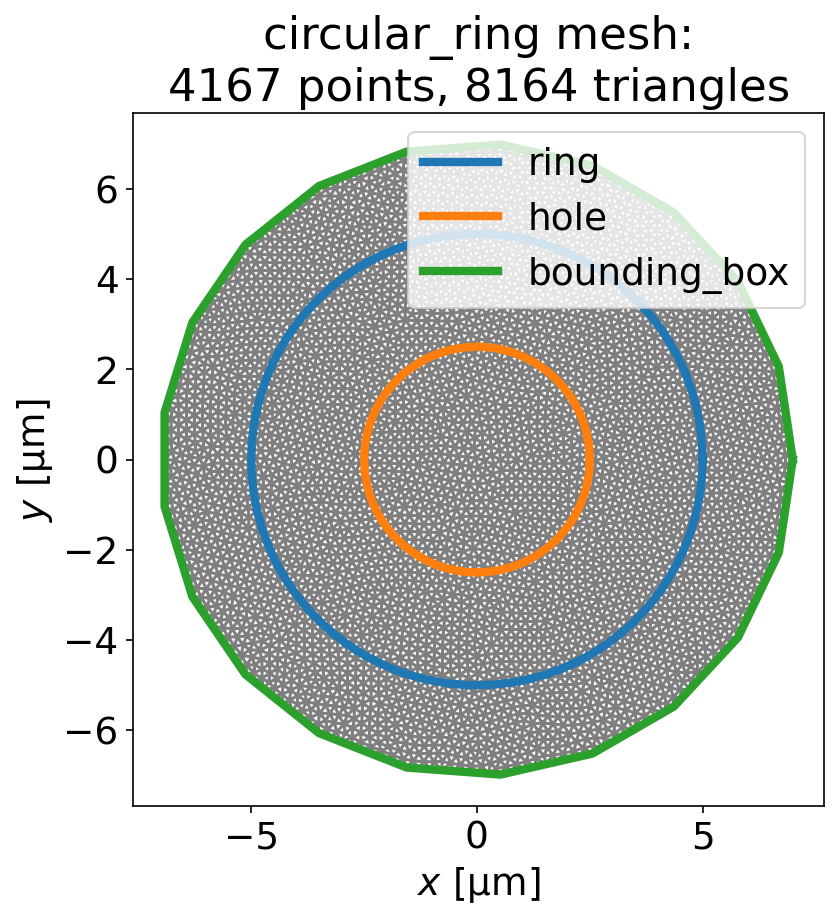
\includegraphics[width=\linewidth]{examples/images/ring/circular_ring_mesh.png}
  \caption{Circular ring, \mintinline{python}{optimesh_steps=400}.}
  \label{fig:circular_ring_mesh}
\end{subfigure}%
\begin{subfigure}{.4\textwidth}
  \centering
  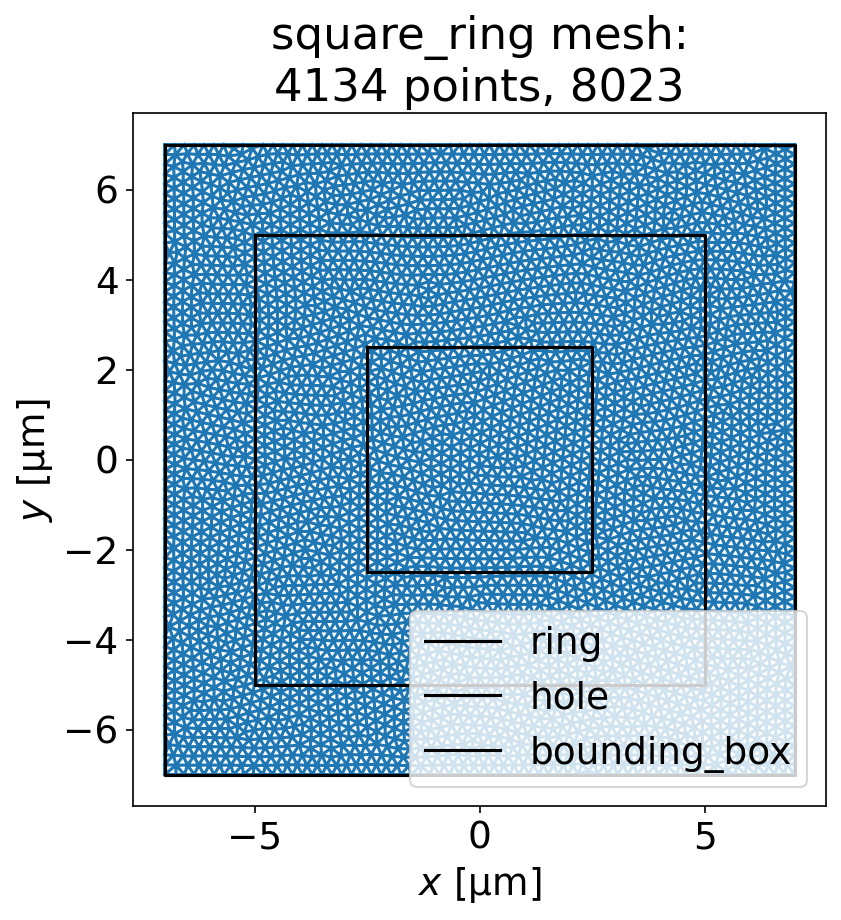
\includegraphics[width=\linewidth]{examples/images/ring/square_ring_mesh.png}
  \caption{Square ring, \mintinline{python}{optimesh_steps=400}.}
  \label{fig:square_ring_mesh}
\end{subfigure}
\begin{subfigure}{.4\textwidth}
  \centering
  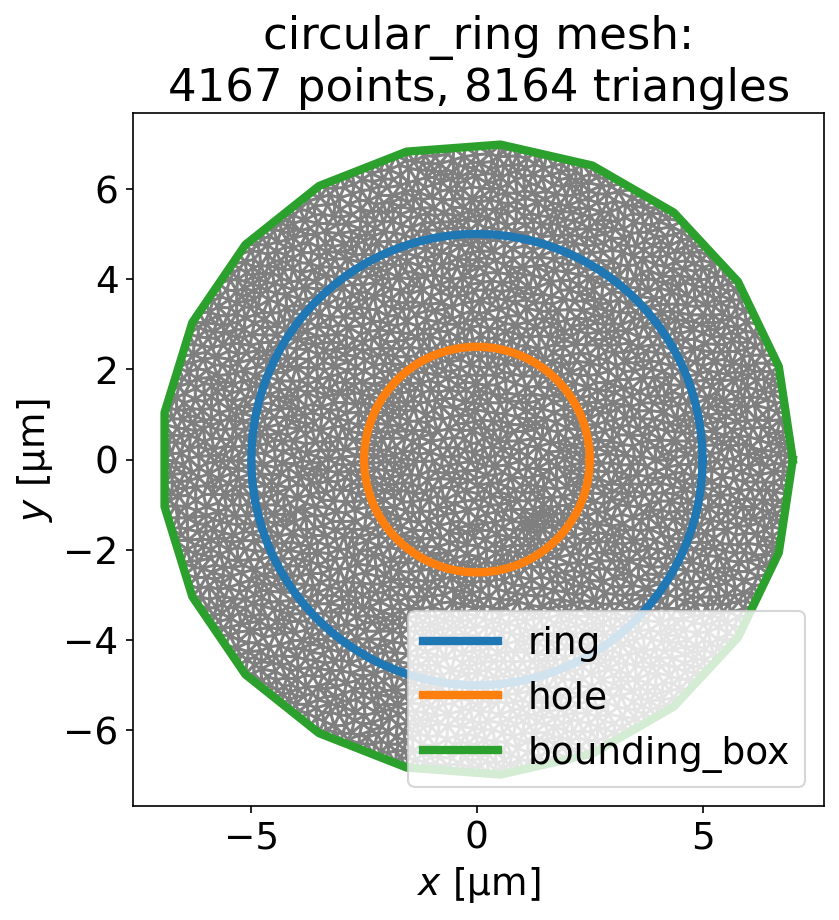
\includegraphics[width=\linewidth]{examples/images/ring/circular_ring_mesh_no_optimesh.png}
  \caption{Circular ring, \mintinline{python}{optimesh_steps=None}.}
  \label{fig:circular_ring_mesh_no_opt}
\end{subfigure}%
\begin{subfigure}{.4\textwidth}
  \centering
  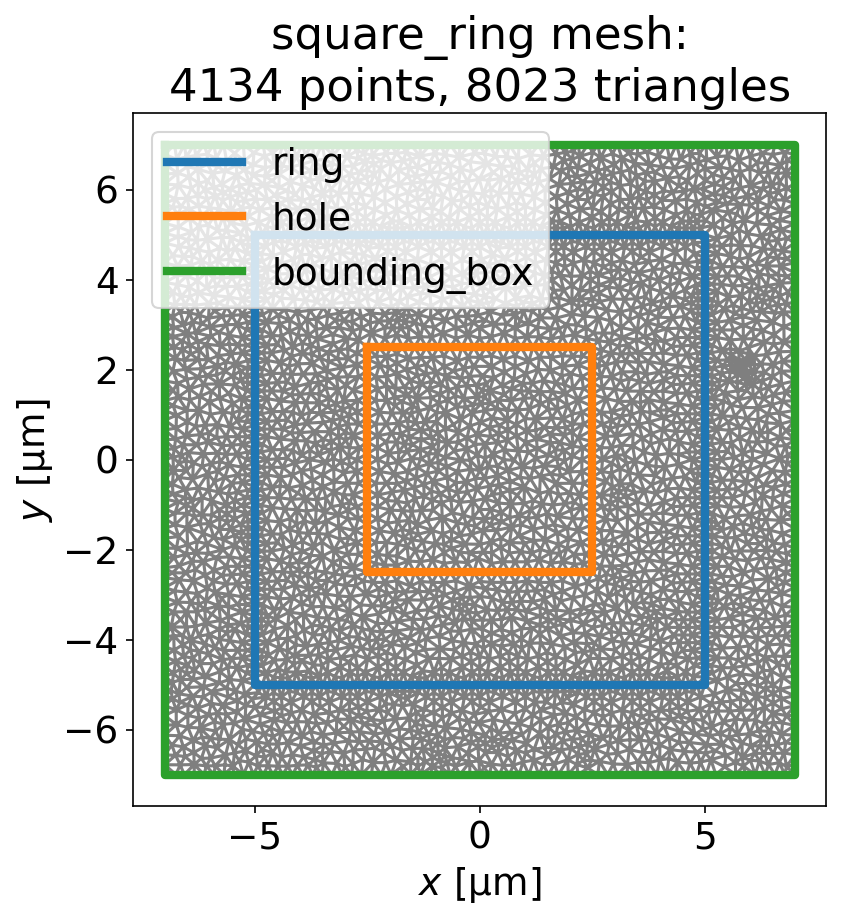
\includegraphics[width=\linewidth]{examples/images/ring/square_ring_mesh_no_optimesh.png}
  \caption{Square ring, \mintinline{python}{optimesh_steps=None}.}
  \label{fig:square_ring_mesh_no_opt}
\end{subfigure}
\caption{Device geometry and mesh for a circular and square ring generated using Code Blocks~\ref{code:device} and \ref{code:mesh_generation}, with (top row) and without (bottom row) \mintinline{python}{optimesh} optimization.}
\label{fig:ring_mesh}
\end{figure}

After the mesh is generated, the matrices and vectors described in Section~\ref{section:implementation} can be computed and one can begin solving models.

\subsection{Solvers}
\label{section:overview:solvers}

A \SuperScreen model consists of a \mintinline{python}{Device}, a function or \mintinline{python}{Parameter} that defines the applied magnetic field as a function of position $H_{z,\,\mathrm{applied}}(x, y, z)$, and a value for the current circulating around each hole in the device due to trapped flux (if any). These items serve as the inputs to \SuperScreen's main solver function, \mintinline{python}{superscreen.solve()}, which implements the calculation outlined in Section~\ref{section:implementation}. When simulating a device with more than one layer, one can specify the number of times to implement the iterative calculation described in Section~\ref{section:model:multilayer} in order to solve for the response of all layers self-consistently. One can also skip the iterative portion of the calculation entirely and only solve for the response of each layer to the applied field, assuming no interaction between layers.

For example, Code Block~\ref{code:ring_circulating_current} solves two models involving the \mintinline{python}{ring} device. First, Meissner screening of a spatially uniform applied magnetic field, and second, the response of the ring to trapped flux with an associated circulating current of 1 mA with no applied magnetic field. The resulting sheet current and magnetic field distributions can be visualized using the \mintinline{python}{plot_current()} and \mintinline{python}{plot_fields()} methods, which produce the images shown in Figure~\ref{fig:ring_plot_fields_currents}.

\begin{code}
\begin{minted}[fontsize=\footnotesize]{python}
# Simulate the response to a uniform applied field of 0.2 mT
applied_field = sc.sources.ConstantField(0.2)
field_units = "mT"

solutions = sc.solve(
    device=ring,
    applied_field=applied_field,
    field_units=field_units,
)
assert len(solutions) == 1 # Since there is only one layer
uniform_field = solutions[-1]

# Simulate a current circulating around the hole in the ring.
circulating_currents = {"hole": "1 mA"}

solutions = sc.solve(
    device=ring,
    applied_field=None,
    circulating_currents=circulating_currents
)
assert len(solutions) == 1 # Since there is only one layer
trapped_flux = solutions[-1]

for solution in (uniform_field, trapped_flux):
    solution.plot_currents(
        figsize=(6, 7), cross_section_ys=[0], units="mA/um",
    )
    solution.plot_fields(figsize=(6, 7), cross_section_ys=[0])
\end{minted}
\captionof{listing}{Solve for the current and magnetic field distributions resulting from a total current of 1 mA flowing in our \mintinline{python}{ring} device.}
\label{code:ring_circulating_current}
\end{code}

% \begin{code}
% \begin{minted}[fontsize=\footnotesize]{python}
% # Simulate a current circulating around the hole in the ring.
% circulating_currents = {"hole": "1 mA"}

% solutions = sc.solve(
%     device=ring,
%     applied_field=None,
%     circulating_currents=circulating_currents
% )
% assert len(solutions) == 1 # Since there is only one layer
% solution = solutions[-1]

% solution.plot_currents(
%     figsize=(6, 7), cross_section_ys=[0], units="mA/um",
% )

% solution.plot_fields(
%     figsize=(6, 7), cross_section_ys=[0],
% )
% \end{minted}
% \captionof{listing}{Solve for the current and magnetic field distributions resulting from a total current of 1 mA flowing in our \mintinline{python}{ring} device.}
% \label{code:ring_circulating_current}
% \end{code}

\begin{figure}
\centering
\begin{subfigure}{.4\textwidth}
  \centering
  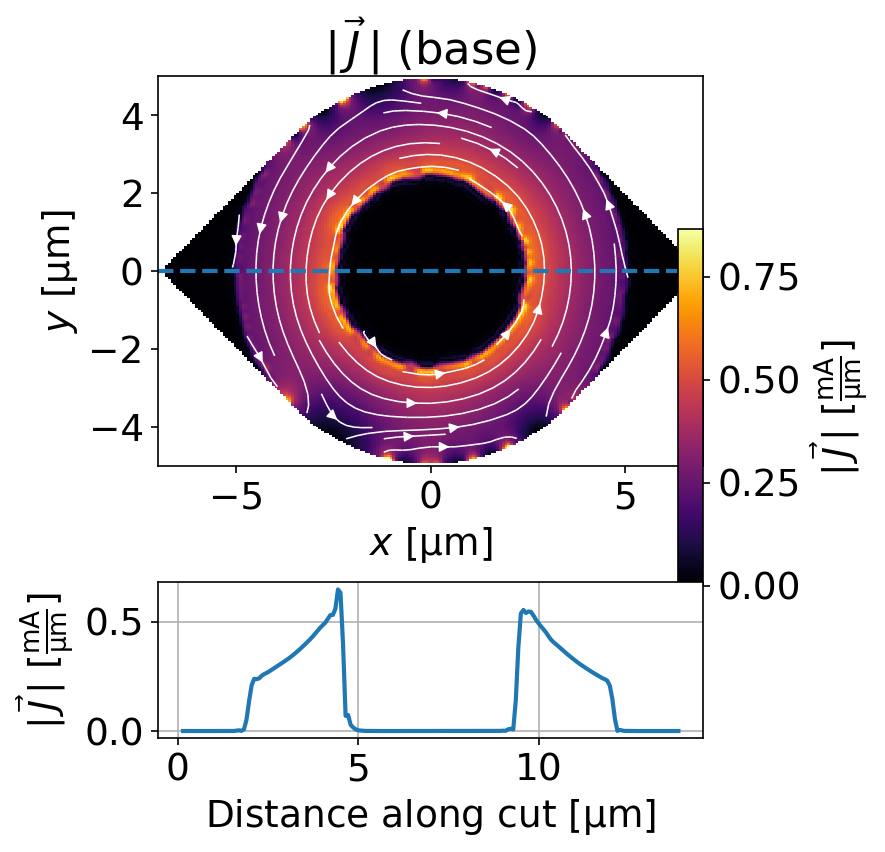
\includegraphics[width=\linewidth]{examples/images/ring/circular_ring_plot_currents.png}
  \caption{Circular ring sheet current.}
  \label{fig:circular_ring_plot_currents}
\end{subfigure}
\begin{subfigure}{.4\textwidth}
  \centering
  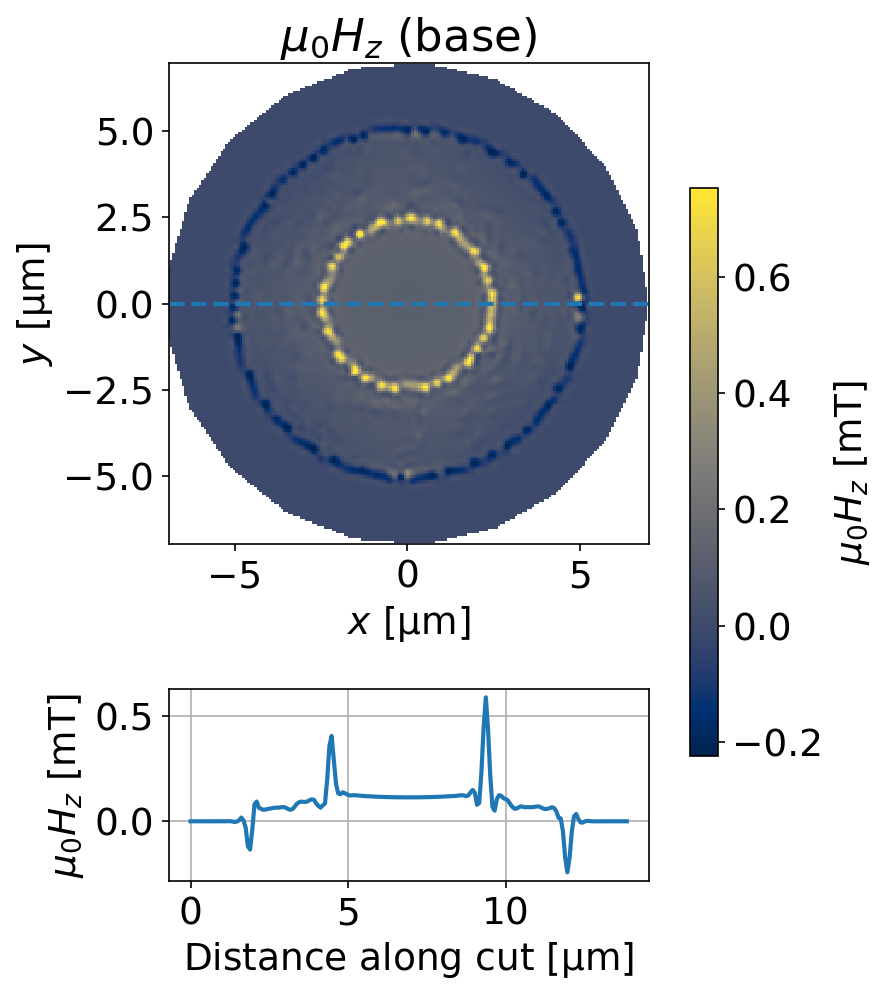
\includegraphics[width=\linewidth]{examples/images/ring/circular_ring_plot_fields.png}
  \caption{Circular ring magnetic field.}
  \label{fig:circular_ring_plot_fields}
\end{subfigure}

\begin{subfigure}{.4\textwidth}
  \centering
  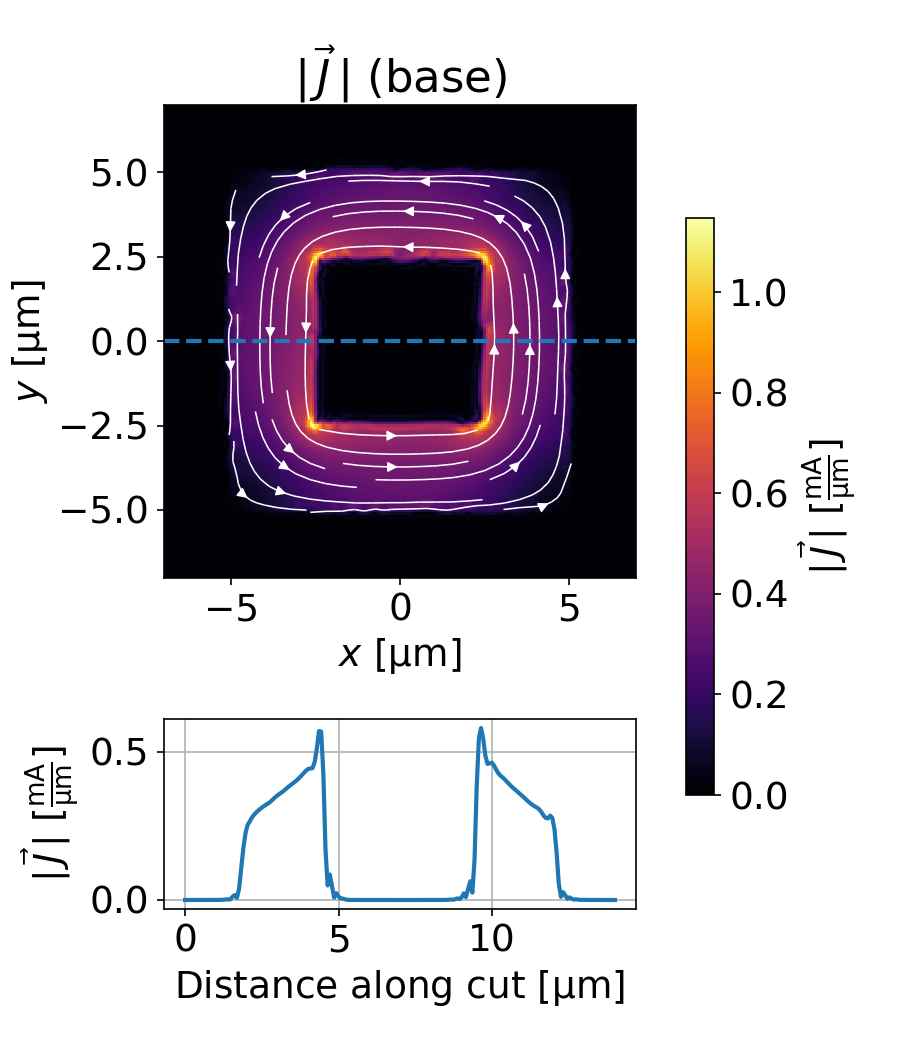
\includegraphics[width=\linewidth]{examples/images/ring/square_ring_plot_currents.png}
  \caption{Square ring sheet current.}
  \label{fig:square_ring_plot_currents}
\end{subfigure}
\begin{subfigure}{.4\textwidth}
  \centering
  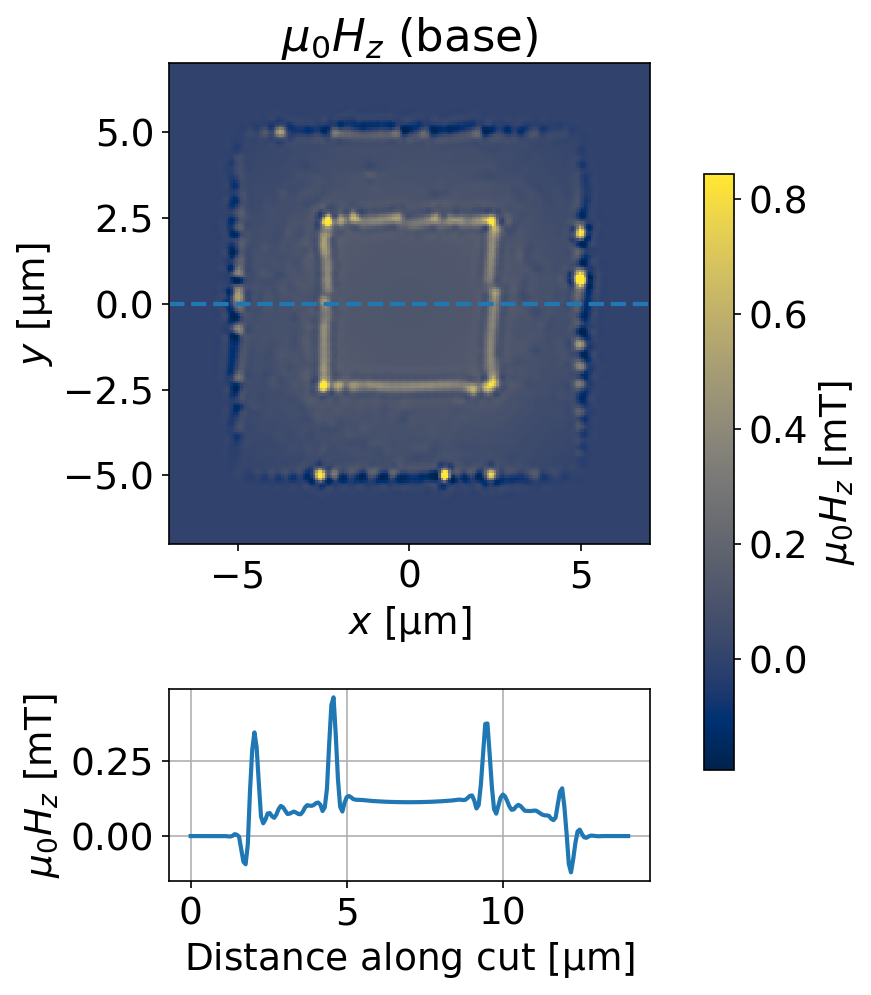
\includegraphics[width=\linewidth]{examples/images/ring/square_ring_plot_fields.png}
  \caption{Square ring magnetic field.}
  \label{fig:square_ring_plot_fields}
\end{subfigure}

\caption{Sheet current $\vec{J}$ and magnetic field $\mu_0H_z$ distributions for the circular (top) and square (bottom) ring calculated using Code Block~\ref{code:ring_circulating_current}.}
\label{fig:ring_circulating_current}
\end{figure}

The output of \mintinline{python}{superscreen.solve()} is a \mintinline{python}{list} of \mintinline{python}{superscreen.Solution} objects, with a length of 1 plus the number of iterations used for the iterative portion of the calculation. A \mintinline{python}{Solution} encapsulates all of the information about a solved model: the \mintinline{python}{Device}, applied field, circulating currents, and calculated stream functions and magnetic fields for all layers in the device. A \mintinline{python}{Solution} also has methods for processing the simulation results, including:
\begin{itemize}
    \item{
    \mintinline{python}{Solution.grid_data()}: Interpolates the calculated stream functions and magnetic fields for each layer from the triangular mesh to a rectangular grid.
    }
    \item{
    \mintinline{python}{Solution.current_density()}: Interpolates the stream functions to a rectangular grid and calculates the current density (sheet current) $\vec{J}(x, y)$ in each layer using Eq.~\ref{eq:stream}.
    }
    \item{
    \mintinline{python}{Solution.polygon_flux()}: Calculates the total flux through each polygon in the device (films, holes, and abstract regions).
    }
    \item{
    \mintinline{python}{Solution.field_at_position()}: Calculates the vector magnetic field at any point(s) in space due the applied field and the currents flowing the in the device using Eqs.~\ref{eq:field_from_kernel} and \ref{eq:kernels}.
    }
\end{itemize}

One may wish to solve many models involving the same device while varying other aspects of the model, for example sweeping the applied field, circulating currents, or some parameter of one or more layers in the device. Fortunately, the mesh and large matrices described in Section~\ref{section:implementation} depend only on the geometry of the device parallel to the $x-y$ plane. This means that the same mesh and matrices can be re-used for models with different applied fields, circulating currents, layer heights (vertical positions), and penetration depths.

The \mintinline{python}{superscreen.solve_many()} function manages the setup and execution of such a sweep. One can provide a sequence of \mintinline{python}{Parameter} objects defining different applied fields and/or a sequence of circulating current values over which to sweep and/or a ``layer updater" function that modifies each layer in the device according to some set of keyword arguments, which can also be swept. The latter option can be used to sweep layer heights or penetration depths. Given these inputs, \mintinline{python}{superscreen.solve_many()} will generate and solve all of the corresponding models. The models can either be solved in series in a single Python process (the default), or in parallel across multiple Python processes running across multiple CPUs, or even across multiple nodes in a cluster. In any case, only a single copy of the device's mesh and large arrays is created, so the memory overhead is modest.

\subsection{Visualization}
\label{section:overview:visualization}

\SuperScreen offers several functions for visualizing the results of simulations (which are also aliased as methods on \mintinline{python}{superscreen.Solution}):

\begin{itemize}
    \item{
    \mintinline{python}{superscreen.plot_streams()}: Given a \mintinline{python}{Solution}, plots the stream function $g(x, y)$ for one or more layers in the device.
    
    See also: \mintinline{python}{Solution.plot_streams()}.
    }
    \item{
    \mintinline{python}{superscreen.plot_currents()}: Given a \mintinline{python}{Solution}, plots the sheet current $\vec{J}(x, y)$ for one or more layers in the device.
    
    See also: \mintinline{python}{Solution.plot_currents()}.
    }
    \item{
    \mintinline{python}{superscreen.plot_fields()}: Given a \mintinline{python}{Solution}, plots the total field $H_z(x, y)$ or the screening field $H_z(x, y) - H_{z,\,\mathrm{applied}}(x, y)$ for one or more layers in the device.
    
    See also: \mintinline{python}{Solution.plot_fields()}.
    }
    \item{
    \mintinline{python}{superscreen.plot_field_at_positions()}: Given a \mintinline{python}{Solution}, plots the total field $\vec{H}(x, y, z_0)$ or $H_z(x, y, z_0)$ at any points in space (where $z_0$ is not equal to the vertical position of any of the layers in the device).
    
    See also: \mintinline{python}{Solution.plot_field_at_positions()}.
    }
\end{itemize}

See Section~\ref{section:examples} for examples of the figures generated by these functions.

\subsection{Comparison \& Persistence}
\label{section:overview:persistence}

\mintinline{python}{Parameters}, \mintinline{python}{Layers}, \mintinline{python}{Polygons}, \mintinline{python}{Devices}, and \mintinline{python}{Solutions} all implement the equality operator, \mintinline{python}{==}. Two \mintinline{python}{Parameters} are considered equal if the Python bytecode of their underlying functions is the same and their keyword arguments are the same. Two \mintinline{python}{Layers} are equal if their name, penetration depth, thickness, and vertical position are all equal. Two \mintinline{python}{Polygons} are equal if they are in the same layer and their name and polygon vertices are equal. Two \mintinline{python}{Devices} are equal if their name, layers, films, holes, and abstract regions are all equal. Two \mintinline{python}{Solutions} are equal if their device, applied field, circulating currents, timestamp (time at which the solution was created), and all stream function and magnetic field arrays are equal. Two \mintinline{python}{Solutions} created at different times can also be compared by calling \mintinline{python}{solution.equals(other_solution, require_same_timestamp=False)}.

Instances of \mintinline{python}{superscreen.Device} and \mintinline{python}{superscreen.Solution} can be saved to and loaded from disk using their respective \mintinline{python}{to_file()} and \mintinline{python}{from_file()} methods, making it straightforward to share models and simulation results. \mintinline{python}{Layers}, \mintinline{python}{Polygons}, and all metadata are serialized to JSON, a widely-used, human-readable plain text format~\cite{JSON}. Functions and \mintinline{python}{Parameters}, such as those that compute the applied field or penetration depth, are serialized in binary form using \mintinline{python}{dill}~\cite{McKerns}. \mintinline{python}{numpy} arrays, such as the mesh itself and the computed stream functions and fields, are saved in the well-established \mintinline{python}{numpy} \mintinline{python}{npz} file format. A \mintinline{python}{list} of \mintinline{python}{Solutions}, such as that returned by \mintinline{python}{superscreen.solve()} can be saved/loaded all at once using \mintinline{python}{save_solutions()} and \mintinline{python}{load_solutions()}.

\subsection{Development Details}
\label{section:overview:development}

\SuperScreen requires Python version 3.6 or later. The package is located in a public repository on GitHub~\cite{superscreen}, and a suite of unit tests is run automatically via GitHub Actions whenever a change or proposed change (Pull Request) is made to the \mintinline{python}{main} branch of the repository. At the time of writing, the test suite is executed using Python versions 3.6, 3.7, 3.8, and 3.9, and the test coverage is XX\%. Any changes to the \mintinline{python}{main} branch of the repository also trigger an automatic re-build of the online documentation, hosted by Read the Docs at superscreen.readthedocs.io. Stable versions of the package are tagged on GitHub and uploaded to PyPI, the Python Package Index. The source code and documentation are covered by the MIT License.

\SuperScreen has several important dependencies beyond the Python standard library: \mintinline{python}{numpy}~\cite{2020NumPy-Array} and \mintinline{python}{scipy}~\cite{2020SciPy-NMeth} for numerics, \mintinline{python}{pint}~\cite{Grecco} for handling physical units, \mintinline{python}{matplotlib}~\cite{Hunter_2007} for visualization, \mintinline{python}{meshpy}~\cite{Klockner,Shewchuk} and \mintinline{python}{optimesh}~\cite{nico_schlomer_adam_dobrawy_2021} for mesh generation, \mintinline{python}{dill}~\cite{McKerns} for serializing objects to disk and between processes, and \mintinline{python}{ray}~\cite{ray_2018} for parallel processing with shared memory.

\section{Examples}
\label{section:examples}

Below we demonstrate how to solve several different classes of problems using \mintinline{python}{SuperScreen}: screening of and applied magnetic field by a single superconducting film, current distribution and self-inductance of superconducting rings, and mutual inductance of two superconducting rings. The full source code and interactive Jupyter notebooks for each of the examples can be found in the "examples" directory of the GitHub repository accompanying this paper.

\subsection{Screening}
\label{section:example:screening}

Here we simulate Meissner screening of both uniform and non-uniform applied magnetic fields by superconducting films with different geometries and penetration depths. 

\begin{figure}
    \centering
    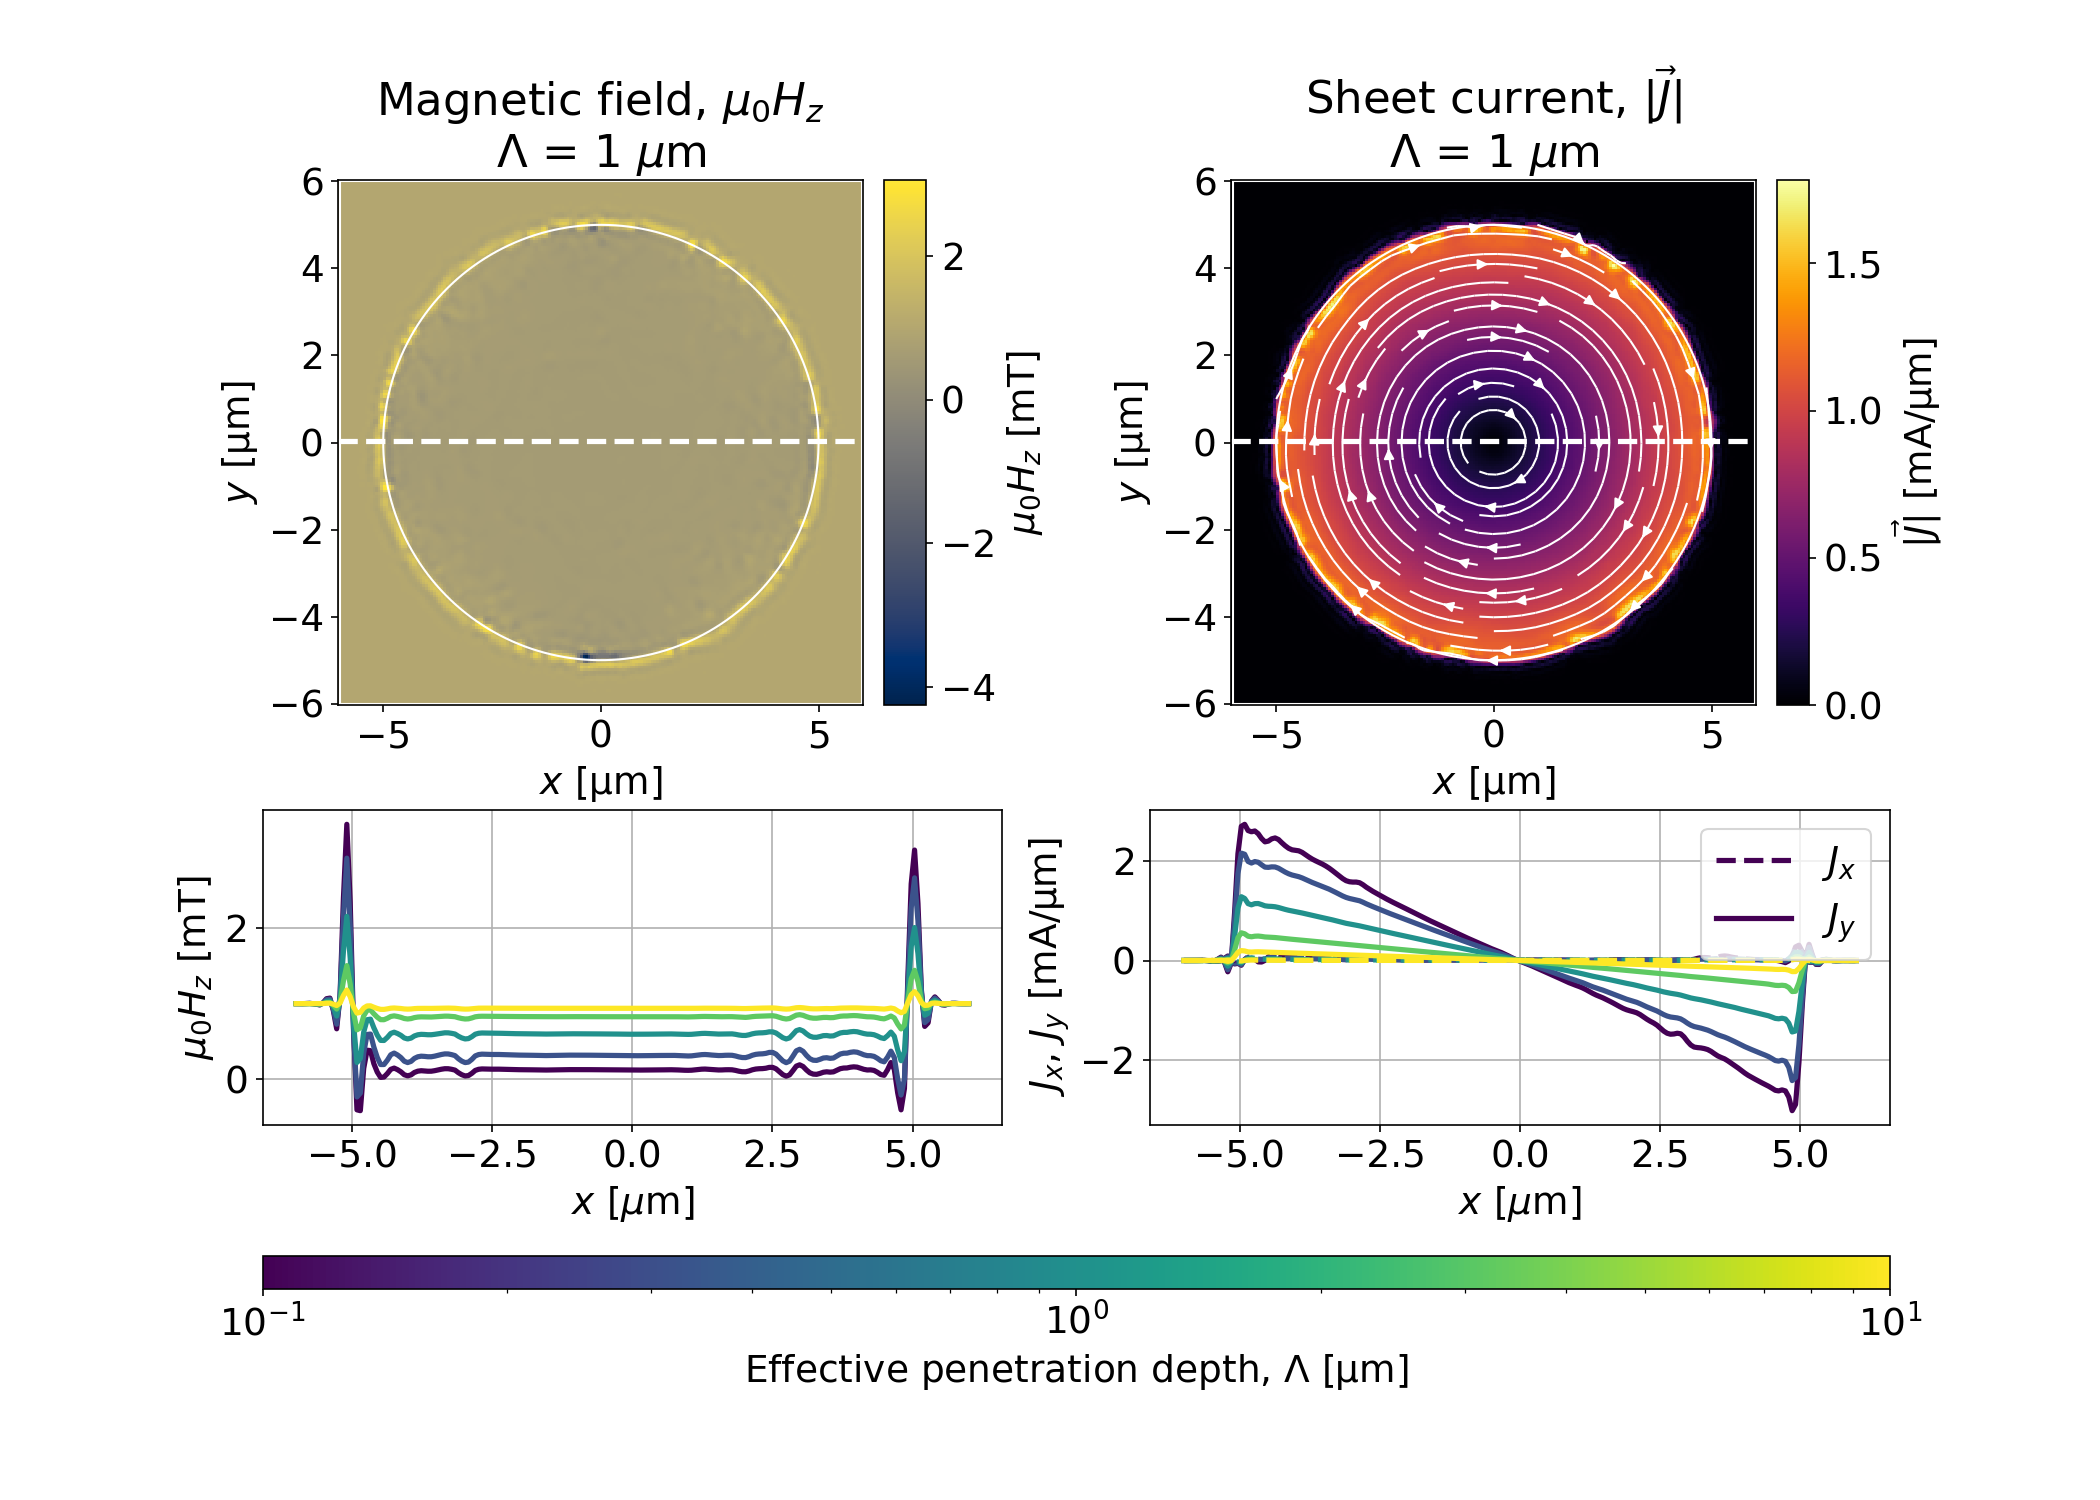
\includegraphics[scale=.40]{examples/images/disk/disk_uniform_field.png}
    \caption{Caption}
    \label{fig:disk_uniform_field}
\end{figure}

\begin{figure}
    \centering
    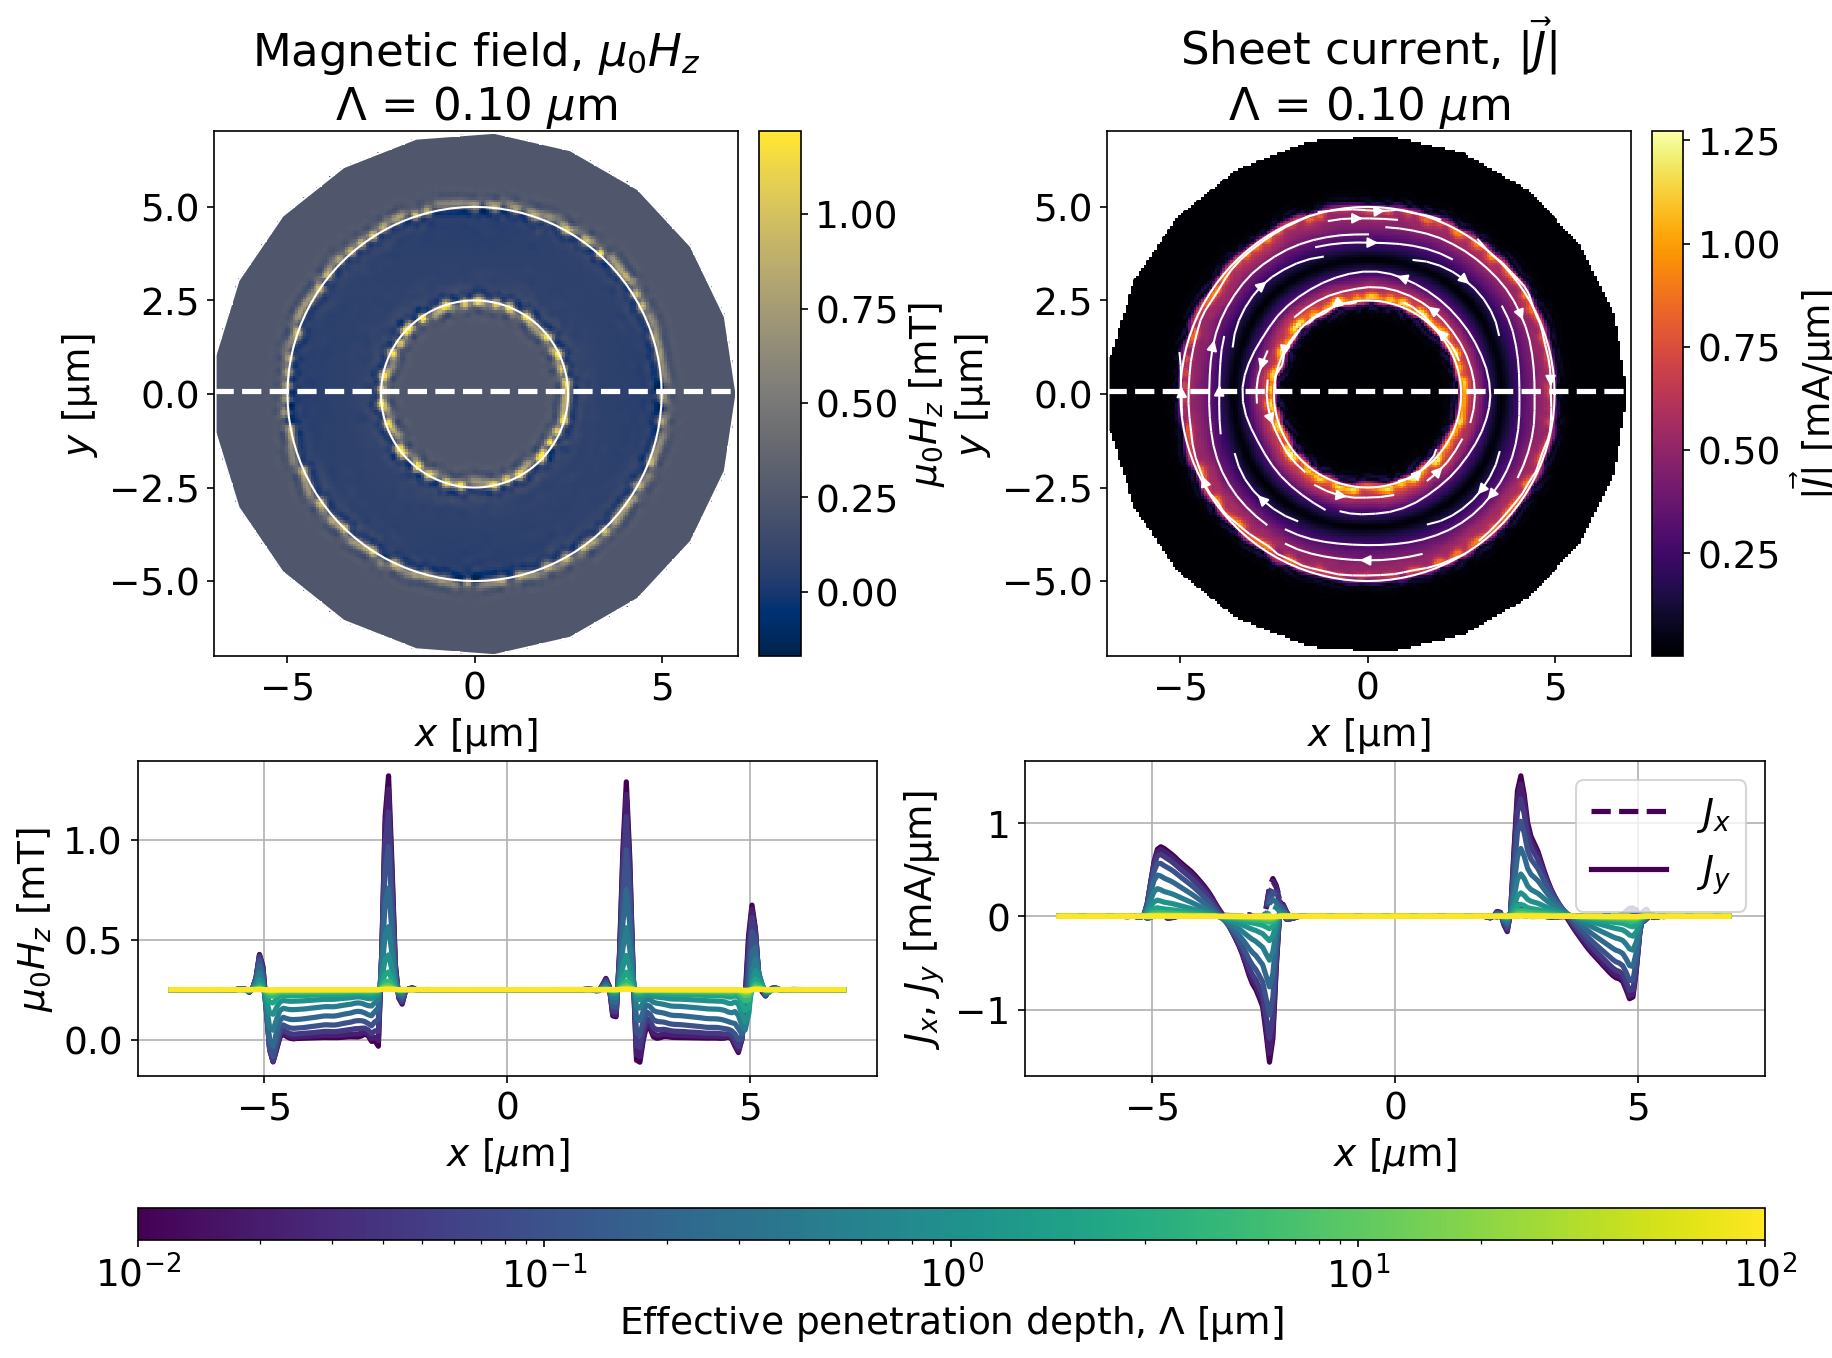
\includegraphics[scale=.40]{examples/images/ring/circular_ring_uniform_field.png}
    \caption{Caption}
    \label{fig:ring_uniform_field}
\end{figure}

\subsection{Self-inductance}
\label{section:examples:inductance}

\begin{figure}
    \centering
    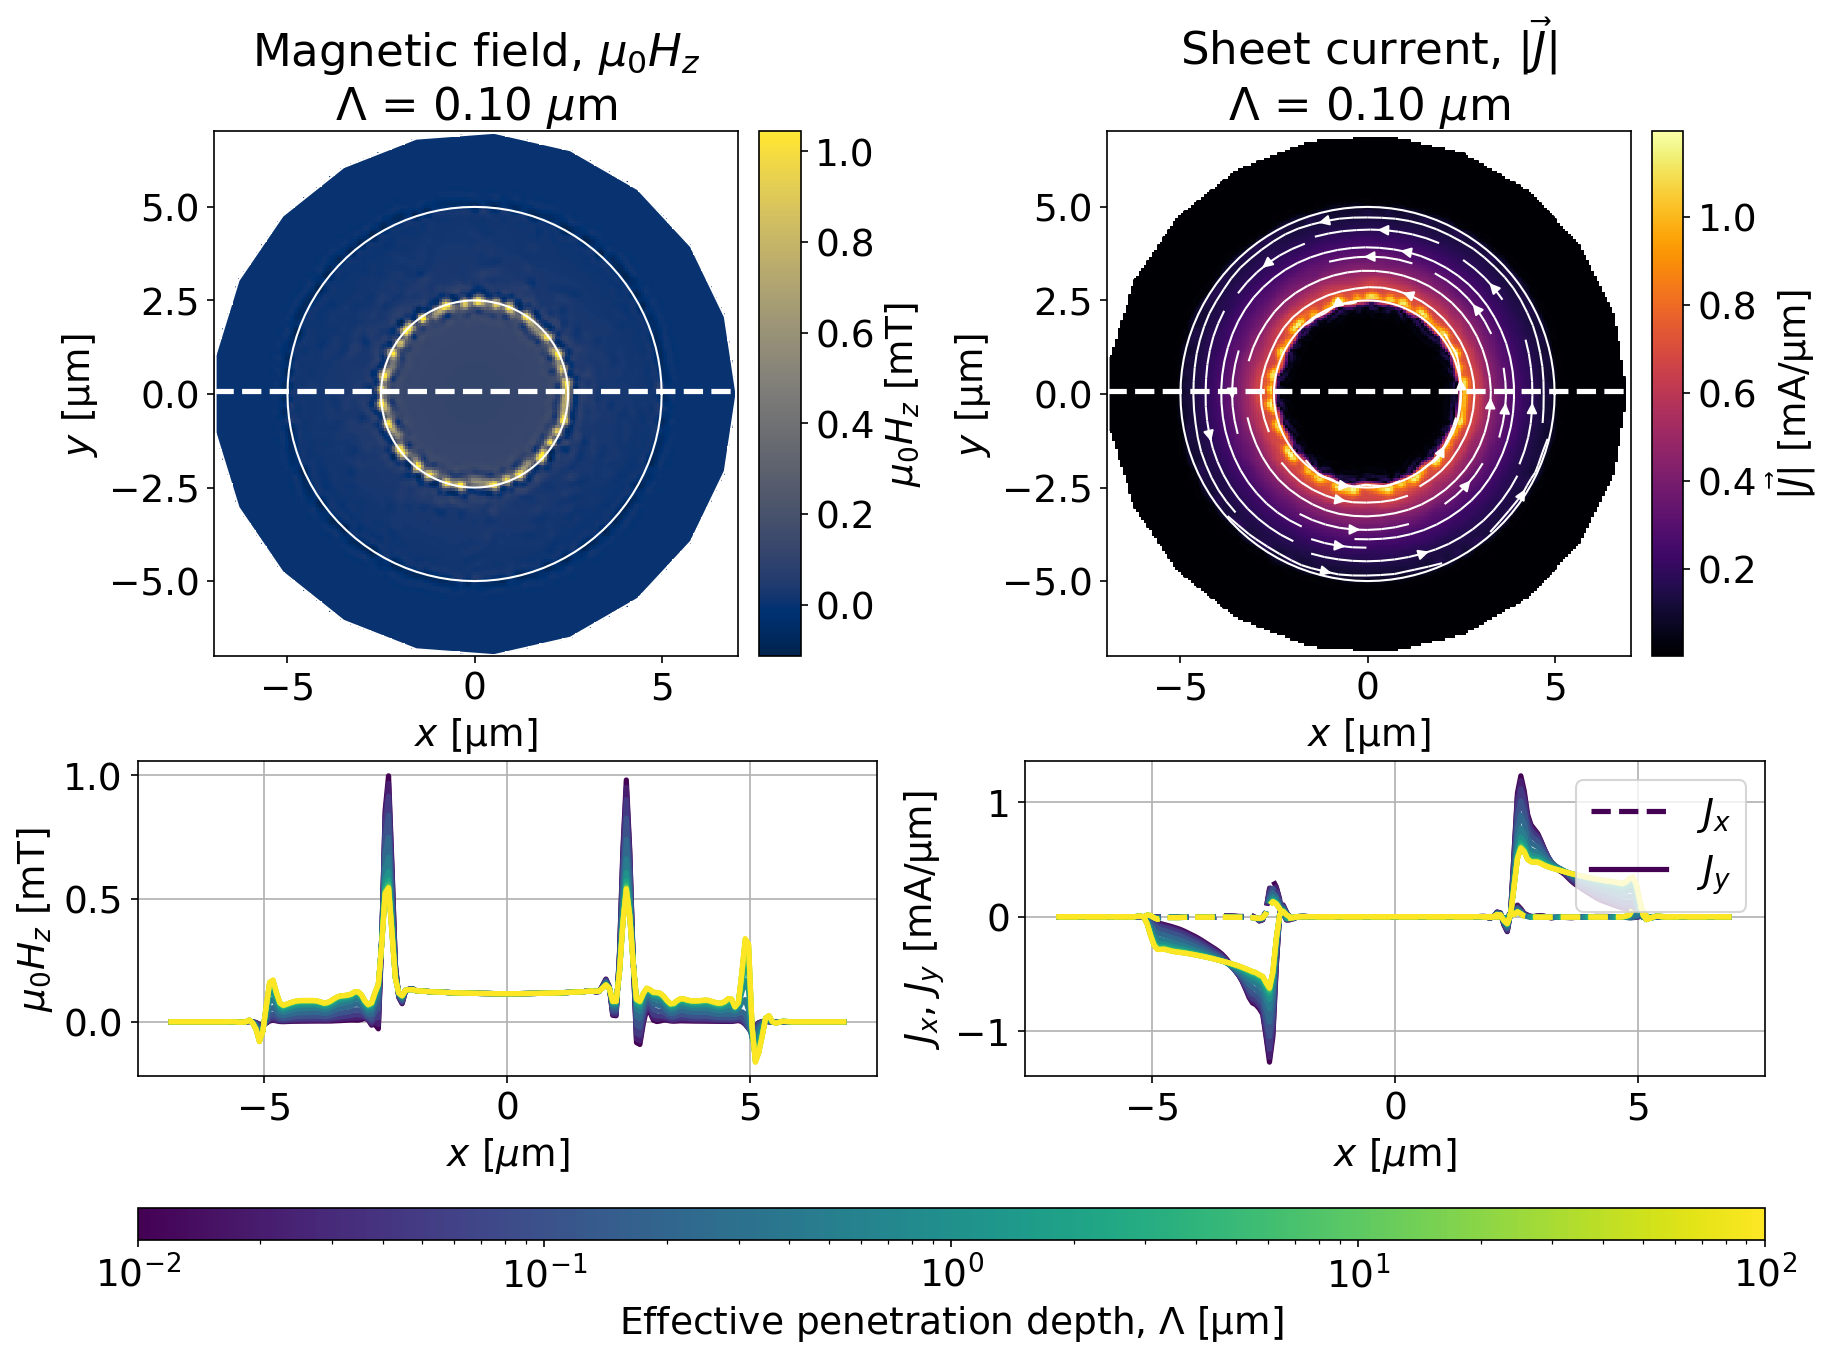
\includegraphics[scale=.40]{examples/images/ring/circular_ring_circulating_current.png}
    \caption{Caption}
    \label{fig:ring_circ_current}
\end{figure}

\begin{figure}
    \centering
    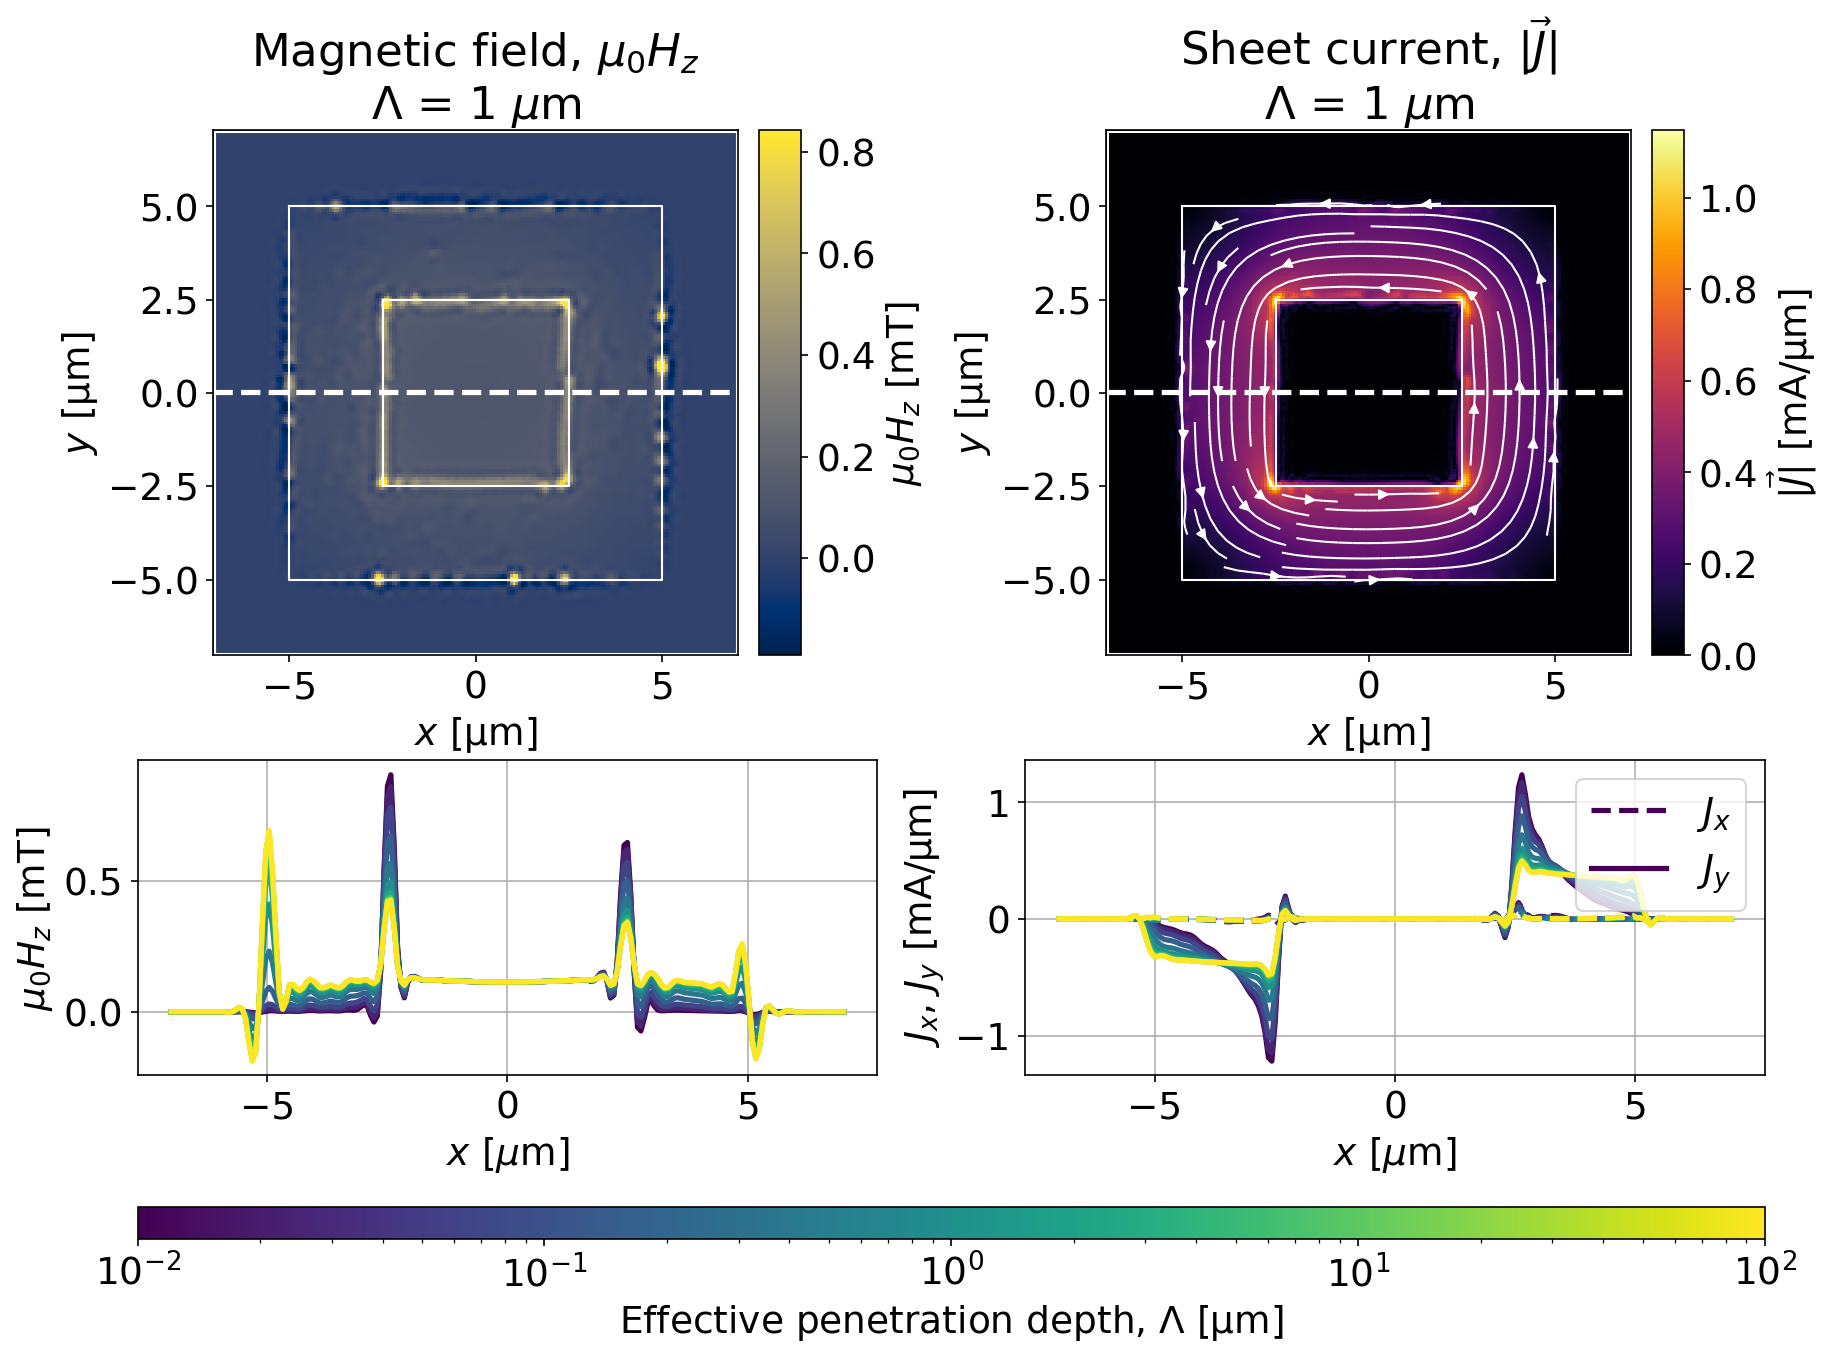
\includegraphics[scale=.40]{examples/images/ring/square_ring_circulating_current.png}
    \caption{Caption}
    \label{fig:square_ring_circ_current}
\end{figure}

\subsection{Mutual Inductance}
\label{section:examples:mutual-inductance}

\subsection{SQUID Susceptometry}
\label{section:examples:susceptometry}

\subsection{Parallel Processing}
\label{section:examples:parallel}


\section{Conclusion}
\label{section:conlusion}

%% The Appendices part is started with the command \appendix;
%% appendix sections are then done as normal sections
%% \appendix

%% \section{}
%% \label{}

%% References
%%
%% Following citation commands can be used in the body text:
%% Usage of \cite is as follows:
%%   \cite{key}         ==>>  [#]
%%   \cite[chap. 2]{key} ==>> [#, chap. 2]
%%

%% References with bibTeX database:

\bibliographystyle{elsarticle-num}
\bibliography{references}

%% Authors are advised to submit their bibtex database files. They are
%% requested to list a bibtex style file in the manuscript if they do
%% not want to use elsarticle-num.bst.

%% References without bibTeX database:

% \begin{thebibliography}{00}

%% \bibitem must have the following form:
%%   \bibitem{key}...
%%

% \bibitem{}

% \end{thebibliography}


\end{document}

%%
%% End of file 